\documentclass[12pt]{article}
\usepackage{geometry} % Pour passer au format A4
\geometry{hmargin=1cm, vmargin=1cm} % 

% Page et encodage
\usepackage[T1]{fontenc} % Use 8-bit encoding that has 256 glyphs
\usepackage[english,french]{babel} % Français et anglais
\usepackage[utf8]{inputenc} 

\usepackage{lmodern}
\setlength\parindent{0pt}

% Graphiques
\usepackage{graphicx,float,grffile}

% Maths et divers
\usepackage{amsmath,amsfonts,amssymb,amsthm,verbatim}
\usepackage{multicol,enumitem,url,eurosym,gensymb}

% Sections
\usepackage{sectsty} % Allows customizing section commands
\allsectionsfont{\centering \normalfont\scshape}

% Tête et pied de page

\usepackage{fancyhdr} 
\pagestyle{fancyplain} 

\fancyhead{} % No page header
\fancyfoot{}

\renewcommand{\headrulewidth}{0pt} % Remove header underlines
\renewcommand{\footrulewidth}{0pt} % Remove footer underlines

\newcommand{\horrule}[1]{\rule{\linewidth}{#1}} % Create horizontal rule command with 1 argument of height

%----------------------------------------------------------------------------------------
%   Début du document
%----------------------------------------------------------------------------------------

\begin{document}

%----------------------------------------------------------------------------------------
% RE-DEFINITION
%----------------------------------------------------------------------------------------
% MATHS
%-----------

\newtheorem{Definition}{Définition}
\newtheorem{Theorem}{Théorème}
\newtheorem{Proposition}{Propriété}

% MATHS
%-----------
\renewcommand{\labelitemi}{$\bullet$}
\renewcommand{\labelitemii}{$\circ$}
%----------------------------------------------------------------------------------------
%   Titre
%----------------------------------------------------------------------------------------

\setlength{\columnseprule}{1pt}

\section*{Le Petit Prince}

\textbf{Le Petit Prince} est un court roman très connu écrit par Antoine de Saint-Exupéry. 
C'est une œuvre poétique et philosophique qui prend l'apparence d'un conte pour enfants. 

\begin{center}
  {\fontfamily{jkplos}\selectfont \og On ne voit bien qu'avec le cœur. L'essentiel est invisible pour les yeux. \fg }\\
  {\fontfamily{jkplos}\selectfont \og C'est le temps que tu as perdu pour ta rose qui fait ta rose si importante. \fg}\\

\end{center}

\subsection*{l’auteur }
\textbf{Antoine de Saint-Exupéry} est né le 29 juin 1900 à Lyon. Il était  écrivain, poète, aviateur et reporter français. Il est mort le 31 juillet 1944. Il était pilote dans l’armée lorsqu’il a disparu en vol au large de Marseille. Il avait refusé la collaboration.

\subsection*{Poèmes}

{\fontfamily{jkplos}\selectfont 

  \subsubsection*{Aviation}

  \begin{verse}
    Les ailes frémissaient sous le souffle du soir \\
	  Le moteur de son chant berçait l'âme endormie \\
	  Le soleil nous frôlait de sa couleur pâle.
  \end{verse}
  
  \subsubsection*{Guerre}
  
  \begin{verse}
	  Parfois confusément sous un rayon lunaire,\\
	  Un soldat se détache incliné sur l'eau claire ; \\
	  il rêve à son amour, il rêve à ses vingt ans !
  \end{verse}
}



\begin{multicols}{2}

  \begin{figure}[H]
        \centering
        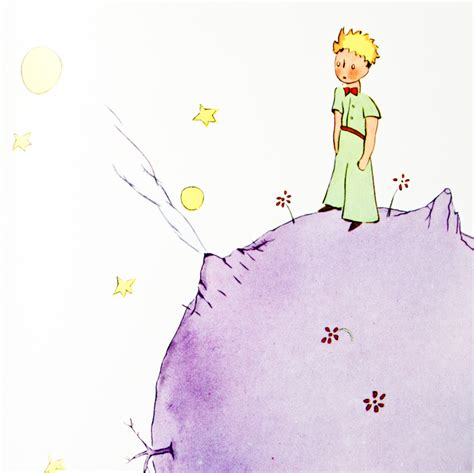
\includegraphics[width=0.9\linewidth]{4x5-calcul-litteral-1/sources/dm-pp.png}
  \end{figure}
\subsection*{En savoir plus}

\begin{itemize}
  \item Wikipedia : \url{https://fr.wikipedia.org/wiki/Le_Petit_Prince}
  \item Wikipedia : \url{https://fr.wikipedia.org/wiki/Antoine_de_Saint-Exup%C3%A9ry}
  \item Site officiel : \url{https://www.lepetitprince.com/}
\end{itemize}


\subsection*{Le petit prince}

On suit un aviateur qui tombe en panne et se pose en catastrophe dans le désert du Sahara. Il n’arrive pas à réparer son avion.
Le lendemain, il est réveillé par un petit personnage qui lui demande : « S'il vous plaît… dessine-moi un mouton ! » 

\end{multicols}
\newpage

\subsection*{Dessine-moi un mouton}

\textit{(Extrait du Petit Prince...)}

\begin{multicols}{2}
  \og S'il vous plaît… dessine-moi un mouton ! \fg \\
  Alors j'ai dessiné.
  
  \begin{figure}[H]
        \centering
        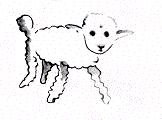
\includegraphics[width=0.3\linewidth]{4x5-calcul-litteral-1/sources/dm-mouton2.png}
  \end{figure}

  Il regarda attentivement, puis: \\
  - Non! Celui-là est déjà très malade. Fais-en un autre. \\
  Je dessinai:

  \begin{figure}[H]
        \centering
        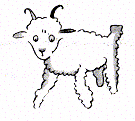
\includegraphics[width=0.3\linewidth]{4x5-calcul-litteral-1/sources/dm-mouton1.png}
  \end{figure}

  Mon ami sourit gentiment, avec indulgence: \\
  - Tu vois bien... ce n'est pas un mouton, c'est un bélier. Il a des cornes... \\
  Je refis donc encore mon dessin:

  \begin{figure}[H]
        \centering
        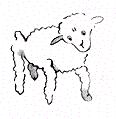
\includegraphics[width=0.3\linewidth]{4x5-calcul-litteral-1/sources/dm-mouton3.png}
  \end{figure}
  
  Mais il fut refusé, comme les précédents: \\
  - Celui-là est trop vieux. Je veux un mouton qui vive longtemps. \\
  Alors, faute de patience, comme j'avais hâte de commencer le démontage de mon moteur, je griffonnai ce dessin-ci.
  
  \begin{figure}[H]
        \centering
        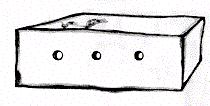
\includegraphics[width=0.5\linewidth]{4x5-calcul-litteral-1/sources/dm-mouton4.png}
  \end{figure}

  Et je lançai: \\
  - Ça c'est la caisse. Le mouton que tu veux est dedans. \\
  Mais je fus bien surpris de voir s'illuminer le visage de mon jeune juge: \\
  - \textbf{C'est tout à fait comme ça que je le voulais ! }
\end{multicols}

\subsection*{Mathématiques}

Il en est de même en mathématiques. Quand nous ne sommes pas sûr de ce que l’on cherche, nous utilisons une "boite à nombre". \textbf{Une boite qui peut contenir le nombre que tu veux}. On appelle cela une inconnue en mathématiques ou encore une variable en informatique. \\

\vspace{2cm}
\centerline{\fontsize{102}{102} $x$}


\end{document}